\documentclass[a4paper,11pt]{article}
\usepackage{amsmath}
\usepackage{graphicx}
\usepackage{float}
\usepackage{url}

\usepackage{verbatim}
\usepackage{listings}
\usepackage{color}

\definecolor{mygreen}{rgb}{0,0.6,0}
\definecolor{mygray}{rgb}{0.5,0.5,0.5}
\definecolor{mymauve}{rgb}{0.58,0,0.82}

\lstdefinelanguage{pseudo}
{
  morekeywords={set,mod,div, if, else, end, to, foreach, then, loop},
  sensitive=false,
  morecomment=[l]{//},
  morecomment=[s]{/*}{*/},
}

\lstset {
 backgroundcolor=\color{white},   % choose the background color; you must add \usepackage{color} or \usepackage{xcolor}
  basicstyle=\footnotesize\ttfamily,        % the size of the fonts that are used for the code
  breakatwhitespace=false,         % sets if automatic breaks should only happen at whitespace
  breaklines=true,                 % sets automatic line breaking
  captionpos=b,                    % sets the caption-position to bottom
  commentstyle=\color{mygreen},    % comment style
  keepspaces=true,                 % keeps spaces in text, useful for keeping indentation of code (possibly needs columns=flexible)
  keywordstyle=\bfseries\color{blue}, % keyword style
  language=pseudo,                 % the language of the code
  numbers=left,                    % where to put the line-numbers; possible values are (none, left, right)
  numbersep=5pt,                   % how far the line-numbers are from the code
  numberstyle=\tiny\color{mygray}, % the style that is used for the line-numbers
  rulecolor=\color{black},         % if not set, the frame-color may be changed on line-breaks within not-black text (e.g. comments (green here))
  showstringspaces=false,          % underline spaces within strings only
  showtabs=false,                  % show tabs within strings adding particular underscores
  stepnumber=1,                    % the step between two line-numbers. If it's 1, each line will be numbered
  stringstyle=\color{mymauve},     % string literal style
  tabsize=2,	                   % sets default tabsize to 2 spaces
}



\usepackage[utf8]{inputenc}




\title{Optimizing Trafic Light algorithms in Urban Street Grids\\
\large Introduction to Computational Science}
\author{Jan Kramer\\Klaas Kliffen}
\date{\today}

\begin{document}

\begin{titlepage}
\maketitle
\thispagestyle{empty}
\begin{abstract}
\textit{
 Abstract
}
\end{abstract}
\medskip\medskip
\begin{figure}[H]
  \centering
  \includegraphics[width=.4\linewidth]{img/trafficlighttree.jpg}
\end{figure}


\end{titlepage}

\newpage
\tableofcontents

\newpage

\section{Introduction}
% TODO: reread this ;)
Waiting is never fun, especially if you have to get somewhere by car and you are encountering a red traffic light.
Sometimes traffic lights work well, but sometimes it yields a green light for an empty lane, while another lane is packed with cars.
This may not only lead to irritation, but also to dangerous situations if someone decides to ignore the traffic light out of frustration with the traffic light switching algorithm.
In addition bad traffic light switching algorithms also affect the flow of traffic on a larger scale than a single traffic light.

Some effort has been put into researching algortihms and into simulating and using machine learning techniques for determining the best possible algorithms.
Instead of using a complex algorithm, this report evaluates the performance of regular time-based approaches and simple loop detection.

\subsubsection*{Outline of this report}
Section \ref{sec:rel} discusses the use of reinforcement learning for traffic light algorithms.
Section \ref{sec:concept} describes the concept of our simulation.
Section \ref{sec:implementation} goes into to implementation details of the concept.
Section \ref{sec:results} describes the testing set-up used and shows the experimental results.
Section \ref{sec:eval} discusses the results and Section \ref{sec:conclusion} concludes.
In the appendix Section \ref{app:rtables} contains tables with statistics for simulations with various parameters.

\section{Related work}\label{sec:rel}


The paper by Wiering \cite{Wiering00} describes a global algorithm for traffic light switching.
This algorithm is based on multi-agent reinforcement learning to minimize the overal waiting time of cars in the city.
Which basically means that the traffic lights strive as a group to minimize the waiting time by finding a good switching algorithm.
Wiering found that in his simulations that a reinforcement learning algorithm can outperform traditional non-adaptable systems.

\section{Concept}\label{sec:concept}

Instead of complex adaptive learning algorithms, simple algorithms are used in this report.
To simplify the calculations and to keep the scope small our simulation will abstract from the reality.
Therefore we place the following restrictions on the simulation.

Firstly the simulation will only consider cars, there is no other traffic and thus no biking lanes or pedestrian lights.
The reason is that car trafic by itself can be made quite complex already.
Secondly to reduce this complexity all cars will be considered all equal.
So there is no difference between a large truck and small car.
We choose this restriction to simplify the implementation.
In addition cars do not have complex behavior, they just drive forward and choose randomly which lane to pick when entering an intersection.

Thirdly we simplify the traffic network, since it normally can take a quite organic shape.
This organic shape is hard to model and often unique to a city.
So the roads will be generalized to a grid, in which each car takes up exactly one grid space.
Time will be discretized by allowing cars one action per time step:
\begin{itemize}
 \item If not in front of light: move forward one space in the current grid if the next grid space is empty, otherwise wait.
 \item If in front of light: move to the next grid space when the light is green, otherwise wait
\end{itemize}


\subsection{Grid of intersections}
In our simulation the real world traffic network is broken down to intersections.
Each intersection consists of a number of lanes for each direction.
And for each lane a destination direction is set.
The intersections and lanes together form a grid of intersections.
When a car passes the traffic light, it passed on to the next intersection.
Each direction of an intersection is connected to another intersection.
This way a car can navigate from one intersection to another and depending on the number of directions a complex graph like structures can be created.

Another restriction in our model is that each intersection has 2 traffic lights per incoming direction.
One for turning left and one for turning right or going straight ahead.
An extra assumption is that the traffic is well behaved, so we do not allow for states at which collisions between cars can happen.
Initially we consider two possible algorithms for the traffic lights and later two variations for each.

\subsection{Algorithms}

For this assignment two different algorithms will be used, namely a simple algorithm and a two-sided algorithm.
Also variants of both algorithms with loop detection are considered by introducing loop-detection for cars.
The primary inputs for these algorithms are a time stamp, along with a variable for setting the amount of time steps for a light to switch.

\subsubsection*{Simple}
The simple algorithm is based on old-fashioned traffic handling by a human in the center of the intersection pointing at the lane which may move.
At each time step, one of the four directions will get the green light and cars can move.
After a given amount of time steps the next direction will be set to green and the current direction set to red.
This results in the following pseudo code:

\begin{lstlisting}
SET direction TO (time stamp DIV switch time) MOD number of directions
SET lights of lanes in direction TO green
\end{lstlisting}


\subsubsection*{Two Sided}
The two sided algorithm uses the fact that two opposing lanes can move at the same time.
Cars moving straight forward or turning right can move at the same time as the cars on the opposing lane moving forward and right.
The same is true for the lane turning left.
This can be expressed in pseudo code as follows:

\begin{lstlisting}
SET direction TO (time stamp DIV switch time) MOD number of directions
SET light of the lane in the direction TO green
SET the light in the opposing lane TO green
\end{lstlisting}

\subsection*{Loop detection}
Detecting cars in a lane can be done with loop detection.
This usually works by detecting the change in an electromagnetic field when a car passes over it.
If a car is detected in a lane, then the algorithm can give that lane a higher priority.
The loop detection can be applied to both of the previous algorithms.
For this, each traffic light need to keep track of additional information, which lanes currently have green light
and at what time stamp the last change happened.
Naturally it also needs to keep track of the front of each lane and whether a car is present in it.

The loop detection variant will keep the lights on red, while it waits for a car to appear.
It will only set lights to green, if the next lanes are not empty, while it cycles through the lanes.
And if the change time has not yet expired, the algorithm needs to check if there are still cars present.
If this is not the case, then a new light change can be scheduled.
The semantics are as follows given in pseudo code:

\begin{lstlisting}
SET direction TO stored direction
IF time stamp - last change time >= switch time THEN
  SET direction TO direction from algorithm
  IF front of lanes are filled THEN
    SET lights of the lanes from the algorithm TO green
    SET last change time TO time stamp
    SET stored direction TO direction
  ELSE
    FOREACH other direction
      IF front of other lanes in direction is filled THEN
        SET lights of that direction TO green
        SET last change time TO time stamp
        SET stored direction TO direction
        END LOOP
ELSE
  IF front of lanes in direction are empty THEN
    SET last change time TO time stamp - switch time
\end{lstlisting}



\section{Implementation}\label{sec:implementation}

Our implementation of this model has a grid of 9 intersections.
Each intersection is connected to 4 others: up, down, left and right direction.
For boundary intersections, a periodic boundary condition is in place where
cars moving out of the grid will reappear on the opposing side of the grid.
The grid layout can be seen in Figure \ref{fig:intersections}.

\begin{figure}[H]
  \centering
  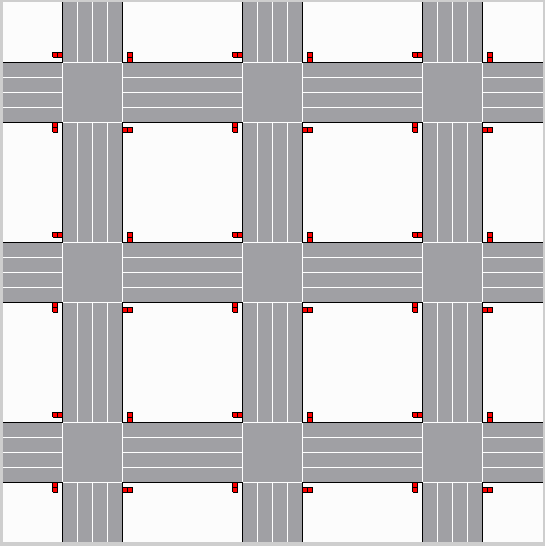
\includegraphics[width=.8\linewidth]{img/intersections.png}
  \caption{The empty intersection grid with all lights red.}
  \label{fig:intersections}
\end{figure}

The code itself is written in the \verb|C++| language \cite{cpp} and the \verb|Qt| framework \cite{qt}.
This allowed us to quickly prototype the model.
Because we simplified the traffic network we can model it as an array of intersections.
Ideally this would be a graph, but this would be too much work currently.
The lanes are then represented by queues for 8 cars, these queues are also stored with arrays.
The most complex code is in the intersection class, which contains all the switching algorithms.
The rest is rather trivial.
Also note that a random numbers generator is used in our application.
While this can reduce the reproducability of the results, this is not the case here because the seed is fixed.
Sadly there is a bug somewhere, so to get reproducable results one has to press the reset button first.
A screenshot of the application can be seen in Figure \ref{fig:screenshot}.

\begin{figure}[H]
  \centering
  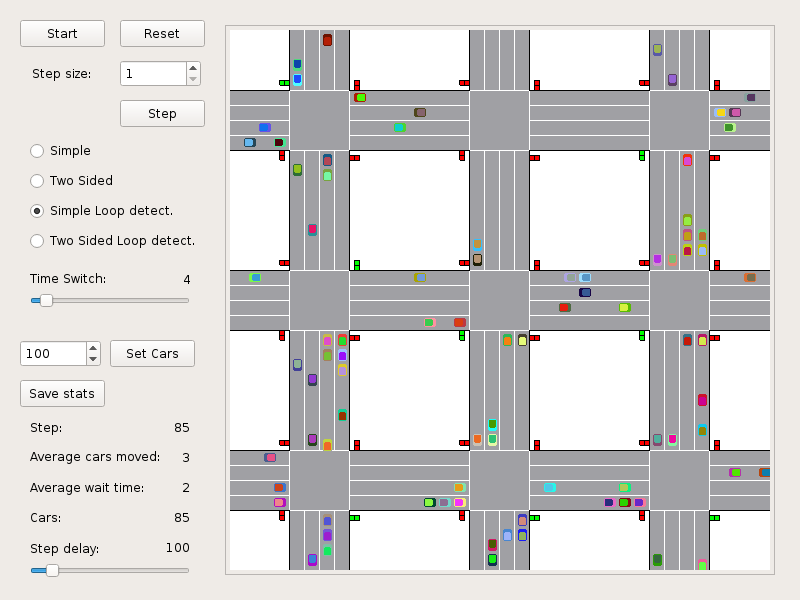
\includegraphics[width=.8\linewidth]{img/screenshot.png}
  \caption{A screenshot of the simulation in action.}
  \label{fig:screenshot}
\end{figure}


\section{Results}\label{sec:results}

For each algorithm we are interested in the performance.
This can for example be measured by keeping track of how many cars flow through the intersection or by how long the waiting times are.
Of course we cannot go measure these things randomly.
An example of the max waiting time can be seen in Figure \ref{fig:waittime}.
As the data is shown the distinction between the two is not immediately clear, since comparing the lines this way is rather hard.

\begin{figure}[H]
  \centering
  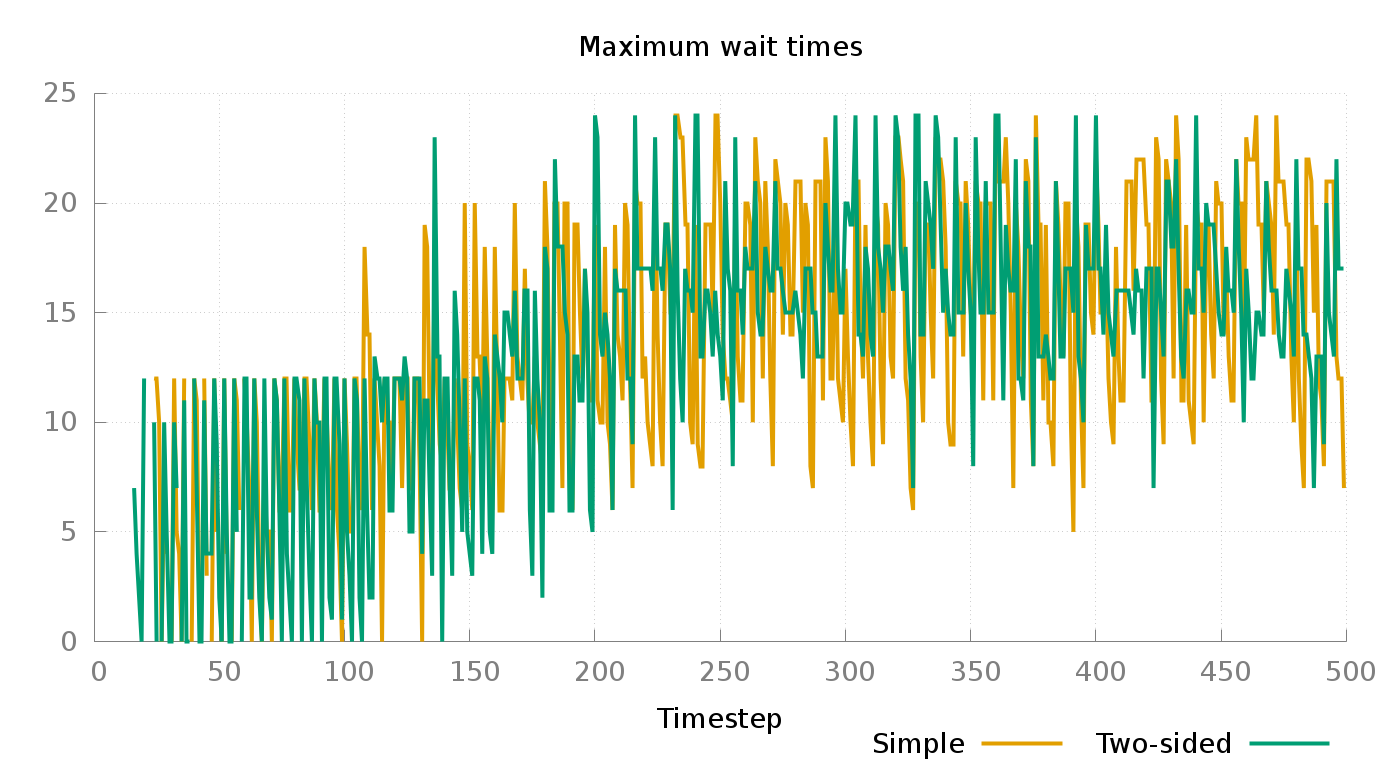
\includegraphics[width=.8\linewidth]{img/maxwait.png}
  \caption{A plot of the maximum waiting times for 200 cars with switching time 4 for algorithms without loop-detection.}
  \label{fig:waittime}
\end{figure}

Another thing to note is that in the beginning the maximum wait time is not yet stable.
Therefore in all our measurements we only use the last $40\%$ of the steps to make sure the system is equilibrium.
To measure the throughput we keep track of how many cars move through the intersection and then average it over the number of steps.
And to measure the waiting times we choose to keep track of the minimum, the maximum and the average waiting time.
As shown in the image above the minimum/maximum waiting times by themselfs are not easy to compare, so we choose to average them.
Note that this is not an entirely realistic measure, since it does not show the spread of the maximum wait times.
We do feel however that this is a good indicator.


Of cource to be able to compare the algorithms not only one situation is enough.
Therefore we varied the number of cars and the switching times.
The number of cars used is: 50, 100 and 200.
By changing the number of cars we try to simulate different densities of traffic.
The different switch times used were: 2, 4, 8, 16 and 32.
These were chosen since they were either a $\frac{1}{4}$, $\frac{1}{2}$, 1, 2 or 4 times the length of the lanes (8) and we expect this to influence the efficientcy of the algorithms.
To make sure that at the end of the simulation it is in an equilibrium state, we ran the simulation for 500 steps.
And to get consistent results, the random generators are seeded with the same seed for each run.

\section{Evaluation}\label{sec:eval}

The resulting statistics can be found in Section \ref{app:rtables} in the appendix.
% TODO: evalution and discussion of the results

\subsubsection*{Patterns}

% TODO: describe the pattern emerging with two sided, long switch time

\section{Conclusion}\label{sec:conclusion}

% TODO: write conclusion

\subsection{Future work}

There is plenty room for improvements on this work in the concept, implementation and the comparison methodology.
The concept can be improved by extending it so that it is more natural.
So one could include other types of traffic or maybe allow for acceleration.
Of course any of the restrictions mentioned in the Concept section could be changed to a situation of interest.
Another interesting effect that could be added is a rush hour effect.
So to model how peaks of high traffic are dealt with.

The implementation could be improved by making it more efficient and more flexible in the sense that it may be nice to handle more and different cars.
One point of interest is the simulation of the traffic.
Currently the lanes the car chooses to go into are choosen at random.
This is not very realistic and maybe the car should have a preset destination it wishes to reach.
The cars then could also have an incentive to drive a certain route.
By making the traffic more realistic we hope that the results of the algorithm also improve.
By moving away from a grid to a graph the distances and the travel time could become more realistic and at the same time allow to test more diverse situations.
One could for example focus on the situation in groningen in particular the find just the right algorithm for their traffic lights.

Lastly the methodology used to compare the algorithms is not perfect.
Take for example the throughput of the intersections.
It may not be independent of the density of the traffic, however just taking the average does not take this in account.
Maybe it should be normalized by the car density or maybe a different statistic altogether makes for a better comparison for example the commulative throughput.
The switching time may also influence the throughput by staying too long on green for example.
This was however not investigated and also not accounted for when we calculated the statistics.
Maybe it is fairer to compare the traffic lights over the same ammount of cycles.

Taking the average of maximum and minimum waiting times also is not a great solution, since we are also interested in the maxima and minima of those.
One possible solution would be to calculate the variance too, so that one could say something about the spread of the values.
However there is this the question if these values also need to be normalized and how.
For example it should probably be normalized for the density of traffic.
So all in all there is plenty left to research.

\bibliographystyle{acm}

\bibliography{refs}

\appendix
\section{Result tables}\label{app:rtables}

\begin{table}[htb]
\centering
\begin{tabular}{cccc}
\hline
\textbf{cars} & 50 & 100 & 200\\
\hline
\textbf{switch time} & & & \\
2 & 0.049751 & 0.21393 & 0.39801 \\
4 & 0.16418 & 0.26368 & 0.50249 \\
8 & 0.19403 & 0.35323 & 0.32836 \\
16 & 0.19403 & 0.33333 & 0.55721 \\
32 & 0.19403 & 0.33333 & 0.25871 \\
\hline
\end{tabular}
\caption{Average minimum queue time for the simple loop algorithm}
\end{table}

\begin{table}[htb]
\centering
\begin{tabular}{cccc}
\hline
\textbf{cars} & 50 & 100 & 200\\
\hline
\textbf{switch time} & & & \\
2 & 1.5822 & 3.301 & 6.9473 \\
4 & 2.0785 & 4.2088 & 7.357 \\
8 & 2.0209 & 4.6099 & 8.8599 \\
16 & 2.0209 & 4.6005 & 9.7013 \\
32 & 2.0209 & 4.6005 & 11.136 \\
\hline
\end{tabular}
\caption{Average queue time for the simple loop algorithm}
\end{table}

\begin{table}[htb]
\centering
\begin{tabular}{cccc}
\hline
\textbf{cars} & 50 & 100 & 200\\
\hline
\textbf{switch time} & & & \\
2 & 3.8408 & 7.9751 & 17.866 \\
4 & 5.0348 & 9.6169 & 16.716 \\
8 & 4.9104 & 10.209 & 19.259 \\
16 & 4.9104 & 10.358 & 22.612 \\
32 & 4.9104 & 10.358 & 29.373 \\
\hline
\end{tabular}
\caption{Average maximum queue time for the simple loop algorithm}
\end{table}

\begin{table}[htb]
\centering
\begin{tabular}{cccc}
\hline
\textbf{cars} & 50 & 100 & 200\\
\hline
\textbf{switch time} & & & \\
2 & 5.4776 & 9.2736 & 13.871 \\
4 & 5.199 & 8.5522 & 13.448 \\
8 & 5.2438 & 8.2388 & 12.214 \\
16 & 5.2438 & 8.2687 & 11.592 \\
32 & 5.2438 & 8.2687 & 10.796 \\
\hline
\end{tabular}
\caption{Average throughput for the simple loop algorithm}
\end{table}


\begin{table}[htb]
\centering
\begin{tabular}{cccc}
\hline
\textbf{cars} & 50 & 100 & 200\\
\hline
\textbf{switch time} & & & \\
2 & 0.089552 & 0.16915 & 0.59204 \\
4 & 0.1592 & 0.39801 & 0.46269 \\
8 & 0.21393 & 0.37811 & 0.60199 \\
16 & 0.21393 & 0.31841 & 0.47761 \\
32 & 0.21393 & 0.31841 & 0.47761 \\
\hline
\end{tabular}
\caption{Average minimum queue time for the two-sided loop algorithm}
\end{table}

\begin{table}[htb]
\centering
\begin{tabular}{cccc}
\hline
\textbf{cars} & 50 & 100 & 200\\
\hline
\textbf{switch time} & & & \\
2 & 1.3433 & 3.1006 & 6.7539 \\
4 & 1.713 & 4.0883 & 7.5746 \\
8 & 1.9167 & 4.6661 & 9.0356 \\
16 & 1.9167 & 4.789 & 9.1792 \\
32 & 1.9167 & 4.789 & 9.1792 \\
\hline
\end{tabular}
\caption{Average queue time for the two-sided loop algorithm}
\end{table}

\begin{table}[htb]
\centering
\begin{tabular}{cccc}
\hline
\textbf{cars} & 50 & 100 & 200\\
\hline
\textbf{switch time} & & & \\
2 & 3.4179 & 7.8159 & 17.204 \\
4 & 4.2786 & 9.0498 & 17.418 \\
8 & 4.6169 & 10.751 & 18.97 \\
16 & 4.6169 & 10.891 & 21.095 \\
32 & 4.6169 & 10.891 & 21.095 \\
\hline
\end{tabular}
\caption{Average maximum queue time for the two-sided loop algorithm}
\end{table}

\begin{table}[htb]
\centering
\begin{tabular}{cccc}
\hline
\textbf{cars} & 50 & 100 & 200\\
\hline
\textbf{switch time} & & & \\
2 & 5.6517 & 9.4478 & 14.03 \\
4 & 5.408 & 8.6219 & 13.274 \\
8 & 5.3134 & 8.2388 & 12.035 \\
16 & 5.3134 & 8.1343 & 11.965 \\
32 & 5.3134 & 8.1343 & 11.965 \\
\hline
\end{tabular}
\caption{Average throughput for the two-sided loop algorithm}
\end{table}

\begin{table}[htb]
\centering
\begin{tabular}{cccc}
\hline
\textbf{cars} & 50 & 100 & 200\\
\hline
\textbf{switch time} & & & \\
2 & 0.54545 & 0.26368 & 0.49254 \\
4 & 2.908 & 3.0955 & 2.8557 \\
8 & 2.88 & 2.75 & 2.5721 \\
16 & 5.2474 & 4.0588 & 4.0546 \\
32 & 19.298 & 9.5122 & 8.1783 \\
\hline
\end{tabular}
\caption{Average minimum queue time for the simple algorithm}
\end{table}

\begin{table}[htb]
\centering
\begin{tabular}{cccc}
\hline
\textbf{cars} & 50 & 100 & 200\\
\hline
\textbf{switch time} & & & \\
2 & 2.8838 & 3.7831 & 6.6417 \\
4 & 6.0868 & 6.8707 & 8.4318 \\
8 & 12.088 & 12.903 & 13.527 \\
16 & 21.503 & 22.225 & 23.952 \\
32 & 52.025 & 47.191 & 48.236 \\
\hline
\end{tabular}
\caption{Average queue time for the simple algorithm}
\end{table}

\begin{table}[htb]
\centering
\begin{tabular}{cccc}
\hline
\textbf{cars} & 50 & 100 & 200\\
\hline
\textbf{switch time} & & & \\
2 & 4.3889 & 8.5721 & 17.139 \\
4 & 6.8712 & 9.5377 & 15.498 \\
8 & 13.51 & 14 & 17.876 \\
16 & 17.423 & 17.662 & 19.53 \\
32 & 35.553 & 30.878 & 30.318 \\
\hline
\end{tabular}
\caption{Average maximum queue time for the simple algorithm}
\end{table}

\begin{table}[htb]
\centering
\begin{tabular}{cccc}
\hline
\textbf{cars} & 50 & 100 & 200\\
\hline
\textbf{switch time} & & & \\
2 & 4.796 & 8.8557 & 14.109 \\
4 & 3.6667 & 6.9254 & 12.502 \\
8 & 2.5423 & 4.8806 & 9.5572 \\
16 & 1.7711 & 3.4428 & 6.5174 \\
32 & 0.801 & 1.7214 & 3.4726 \\
\hline
\end{tabular}
\caption{Average throughput for the simple algorthm}
\end{table}

\begin{table}[htb]
\centering
\begin{tabular}{cccc}
\hline
\textbf{cars} & 50 & 100 & 200\\
\hline
\textbf{switch time} & & & \\
2 & 0.54545 & 0.26368 & 0.49254 \\
4 & 2.908 & 3.0955 & 2.8557 \\
8 & 2.88 & 2.75 & 2.5721 \\
16 & 5.2474 & 4.0588 & 4.0546 \\
32 & 19.298 & 9.5122 & 8.1783 \\
\hline
\end{tabular}
\caption{Average minimum queue time for the two-sided algorithm}
\end{table}

\begin{table}[htb]
\centering
\begin{tabular}{cccc}
\hline
\textbf{cars} & 50 & 100 & 200\\
\hline
\textbf{switch time} & & & \\
2 & 2.8838 & 3.7831 & 6.6417 \\
4 & 6.0868 & 6.8707 & 8.4318 \\
8 & 12.088 & 12.903 & 13.527 \\
16 & 21.503 & 22.225 & 23.952 \\
32 & 52.025 & 47.191 & 48.236 \\
\hline
\end{tabular}
\caption{Average queue time for the two-sided algorithm}
\end{table}

\begin{table}[htb]
\centering
\begin{tabular}{cccc}
\hline
\textbf{cars} & 50 & 100 & 200\\
\hline
\textbf{switch time} & & & \\
2 & 4.3889 & 8.5721 & 17.139 \\
4 & 6.8712 & 9.5377 & 15.498 \\
8 & 13.51 & 14 & 17.876 \\
16 & 17.423 & 17.662 & 19.53 \\
32 & 35.553 & 30.878 & 30.318 \\
\hline
\end{tabular}
\caption{Average maximum queue time for two-sided algorithm}
\end{table}

\begin{table}[htb]
\centering
\begin{tabular}{cccc}
\hline
\textbf{cars} & 50 & 100 & 200\\
\hline
\textbf{switch time} & & & \\
2 & 4.796 & 8.8557 & 14.109 \\
4 & 3.6667 & 6.9254 & 12.502 \\
8 & 2.5423 & 4.8806 & 9.5572 \\
16 & 1.7711 & 3.4428 & 6.5174 \\
32 & 0.801 & 1.7214 & 3.4726 \\
\hline
\end{tabular}
\caption{Average throughput for the two-sided algorithm}
\end{table}

\end{document}
